\documentclass[conference]{IEEEtran}
\IEEEoverridecommandlockouts
% The preceding line is only needed to identify funding in the first footnote. If that is unneeded, please comment it out.
\usepackage{cite}
\usepackage{amsmath,amssymb,amsfonts}
\usepackage{algorithmic}
\usepackage{graphicx}
\usepackage{textcomp}
\usepackage{xcolor}
\usepackage{enumerate}
\usepackage{tabularx}
\usepackage[most]{tcolorbox}
\usepackage{comment}
\usepackage{listings}

\definecolor{codegreen}{rgb}{0,0.6,0}
\definecolor{codegray}{rgb}{0.5,0.5,0.5}
\definecolor{codepurple}{rgb}{0.58,0,0.82}
\definecolor{backcolor}{rgb}{0.95,0.95,0.92}



\lstdefinestyle{mystyle}{
    backgroundcolor=\color{backcolor},   
    commentstyle=\color{codegreen},
    keywordstyle=\color{magenta},
    numberstyle=\tiny\color{codegray},
    stringstyle=\color{codepurple},
    basicstyle=\ttfamily\footnotesize,
    breakatwhitespace=false,         
    breaklines=true,                 
    captionpos=b,                    
    keepspaces=true,                 
    numbers=left,                    
    numbersep=5pt,                  
    showspaces=false,                
    showstringspaces=false,
    showtabs=false,                  
    tabsize=2
}

\lstset{style=mystyle}
\def\BibTeX{{\rm B\kern-.05em{\sc i\kern-.025em b}\kern-.08em
    T\kern-.1667em\lower.7ex\hbox{E}\kern-.125emX}}
\begin{document}

\title{Developing a Test Suite for Evaluating IEC 61499 Application Portability  \\


}

\author{

\IEEEauthorblockN{Midhun Xavier\IEEEauthorrefmark{1}, Tatiana Laikh\IEEEauthorrefmark{1},  Sandeep Patil\IEEEauthorrefmark{1}, Valeriy Vyatkin\IEEEauthorrefmark{1} \IEEEauthorrefmark{3} 
}

\IEEEauthorblockA{\IEEEauthorrefmark{1} Department of Computer Science, Computer and Space Engineering, Lulea Tekniska Universitet, Sweden}



\IEEEauthorblockA{\IEEEauthorrefmark{3}Department of Electrical Engineering and Automation,
Aalto University, Espoo, Finland}



\\ Email: midhun.xavier@ltu.se, tatiana.laikh@ltu.se, sandeep.patil@ltu.se, vyatkin@ieee.org
}



 \maketitle 

\begin{abstract}

This paper presents the creation of a series of function blocks with the specific aim of testing the portability of IEC 61499 applications across diverse development and runtime environments. These function blocks have been developed to cover a wide range of test scenarios, including basic data types, functions, boundary conditions, and adapter features. The function blocks can be conveniently exported or imported through the use of XML files, thus facilitating seamless testing. By testing the runtime environment of different IEC 61499 systems, these function blocks help to identify and highlight any possible issues that may arise related to portability.


%%The proposed standard test function blocks provide a robust tool for developers to evaluate the portability and improve the fault-free development of industrial control system software based on the IEC 61499 standard.

\end{abstract}

\begin{IEEEkeywords}
Industrial Control System, IEC 61499, Testing, Portability
\end{IEEEkeywords}

\section{Testing IEC 61499 Applications: Ensuring Portability Across Different Environments}

The IEC 61499 standard \cite{iec61499part12012} has been developed to address the increasing demands for decentralized control and the exponential growth of control complexity in industrial automation systems, with the aim of establishing an open, component-oriented, and platform-independent development framework to improve the re-usability, reconfigurability, interoperability, portability \cite{gerber2010does}, and distribution of control software for complex distributed systems. The IEC 61499 technology can be effectively used in the implementation of Intelligent Mechatronic Components and engineering processes, using multiple commercial tools and hardware platforms \cite{patil2013composition}. 

The paper \cite{pang2014portability} highlights the importance of addressing portability issues in existing engineering tools for the IEC 61499 standard in order to achieve better interoperability and efficiency in distributed control systems. Testing IEC 61499 applications for adequate functionality is crucial in guaranteeing their compatibility across various development and runtime environment \cite{hopsu2019portability}. To this end, a function blocks library has been designed for testing the basic data types, functions, and boundary conditions, among other key scenarios. A guideline document has been provided to help developers understand the desired results of testing and to modify the test with new values if necessary. 

By enabling developers to test their IEC 61499 applications for portability using the developed standard testing function blocks, the likelihood of errors can be minimized and the efficiency and effectiveness of distributed industrial control systems can be improved.



\section{Test Function Block Design and Development }
\label{sec:mainSec}



\subsection{Data Type testing FBs}
\begin{figure}[!b]
    \centering
    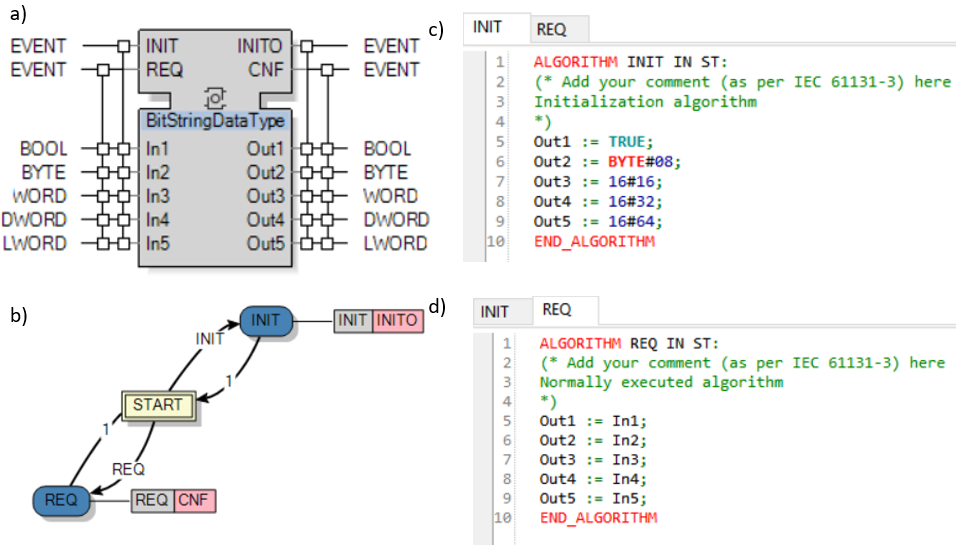
\includegraphics[width=\columnwidth]{Figures/BSDT.PNG}
    \caption{a) BitStringDataType FB interface b) ECC c) INIT Algorithm d) REQ Algorithm.} 
    \label{fig:BSDT}
\end{figure}



\subsubsection{BitStringDataType}

The BitStringDataType function block (FB) is used to test the support of data types and their association for Bit data types, including BOOL, BYTE, WORD, DWORD, and LWORD. The testing procedure for the BitStringDataType FB involves two events, INIT and REQ.

When the INIT event is triggered, the output values of the BitStringDataType FB are set to predefined values. If the output values are not the same as  predefined values then the test fails. This simple test ensures that FB can correctly handle each of the supported data types.

Alternatively, when input data is provided, the REQ event is triggered. The output values of the BitStringDataType FB should correspond to the input values. For example, Out1 should be the same as In1. The CNF event is also triggered by this test. This test ensures that the FB can correctly process the input data and produce the correct output values. The interface, ECC, INIT algorithm, and REQ algorithm for the BitStringDataType function block are depicted in figure \ref{fig:BSDT} a, b, c, and d, respectively.

The BitStringDataType FB is an important testing tool for ensuring that data types and their associations are properly supported in Bit data types. By following the testing procedure outlined above, developers can ensure that their software systems can correctly handle different data types and produce the expected output values.
\hfill \break
\subsubsection{IntegerDataType}

\begin{figure}[!b]
    \centering
    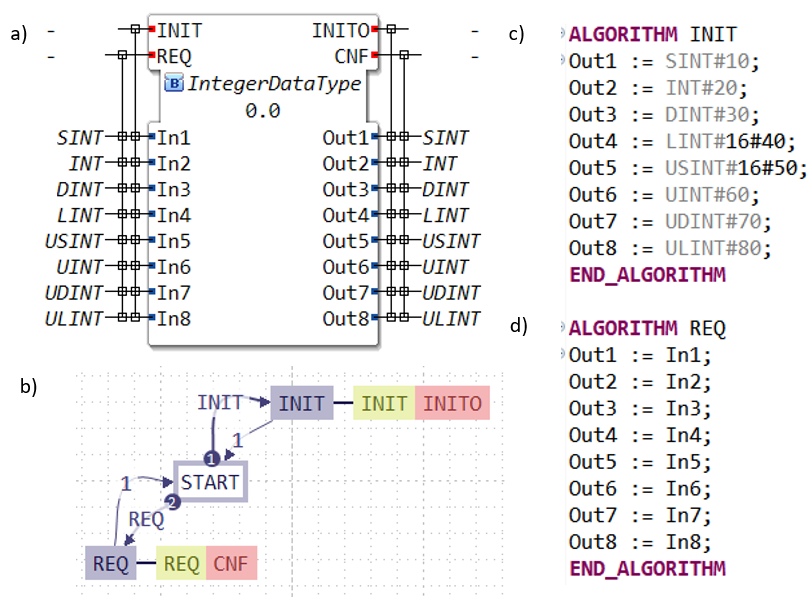
\includegraphics[width=\columnwidth]{Figures/IDT.PNG}
    \caption{a) IntegerDataType FB interface b) ECC c) INIT Algorithm d) REQ Algorithm.} 
    \label{fig:IDT}
\end{figure}

The IntegerDataType function block is used to test the support and association of different integer data types, namely SINT, INT, DINT, LINT, USINT, UINT, UDINT, and ULINT, in an IEC 61499 application. Testing of the IntegerDataType function block can be done in manual mode by triggering the INIT event. When this event is triggered, the output values of Out1 to Out8 should be as follows: 10, 20, 30, 16\#40, 16\#50, 60, 70, and 80. This indicates that the function block correctly supports and associates the specified integer data types.

Another way to test the function block is to add values to the input data and then trigger the REQ event. In this case, the output values of Out1 to Out8 should have the same corresponding values as the input data. For example, the value of Out1 should be the same as the value of In1. This will also trigger the CNF event. These testing procedures help ensure that the IntegerDataType function block works correctly and supports the specified integer data types as expected. IntegerDataType FB interface, ECC, INIT algorithm and REQ algorithm  is shown in figure \ref{fig:IDT} a, b, c and d respectively.
\hfill \break
\subsubsection{RealDataType}

RealDataType also tests similar like the above test FBs.
It is a function block designed for testing the data type support and association with real data types, REAL and LREAL. In the manual testing mode, triggering the INIT event would produce the following output and cause the INITO event to be fired: Out1 with a value of 10.100 and Out2 with a value of 20.2000. Alternatively, as in the case of the BitStringDataType and IntegerDataType test FBs, input data values can be added and the REQ event can be triggered. This would cause the output values to correspond to the input values, such as Out1 being the same as In1. This would also trigger the CNF event.

\subsubsection{StringDataType}

The StringDataType function block (FB) is designed to test the support and association of the STRING data type. In manual testing mode, initiating the INIT event will produce the following output and trigger the INITO event:

Out1 := 'STRING'

Alternatively, adding values to the input data and triggering the REQ event will cause the output values to correspond to the input values. For example, Out1 should match the value of In1. This will also trigger the CNF event.
\break
\subsubsection{TimeDataType, DateDataType, TimeOfDayDataType and DateAndTimeOfDayDataType}

The TimeDataType, DateDataType, TimeOfDayDataType, and DateAndTimeOfDayDataType function blocks (FBs) test the data type support and associations for their respective data types (TIME, LTIME, DATE, LDATE, TIME\_OF\_DAY, LTIME\_OF\_DAY, DATE\_AND\_TIME, and LDATE\_AND\_TIME).

In a manual testing mode, triggering the INIT event will produce output values, and the INITO event will be fired. For TimeDataType, the output values are Out1 := T\#90s15ms and Out2 := LT\#90s15ms542us15ns. For DateDataType, the output values are Out1 := D\#1970-01-01 and Out2 := LD\#2177-11-30. For TimeOfDayDataType, the output values are Out1 := TOD\#00:00:00 and Out2 := LTOD\#00:00:01. For DateAndTimeOfDayDataType, the output values are Out1 := DT\#1970-01-01-00:00:00 and Out2 := LDT\#1971-01-01-00:00:00.

Alternatively, input data can be added and the REQ event can be triggered. The output values should correspond to the input values, and the CNF event will be fired.


\subsection{BoundCheckTest FB}

\begin{figure*}[!t]
	\centering
	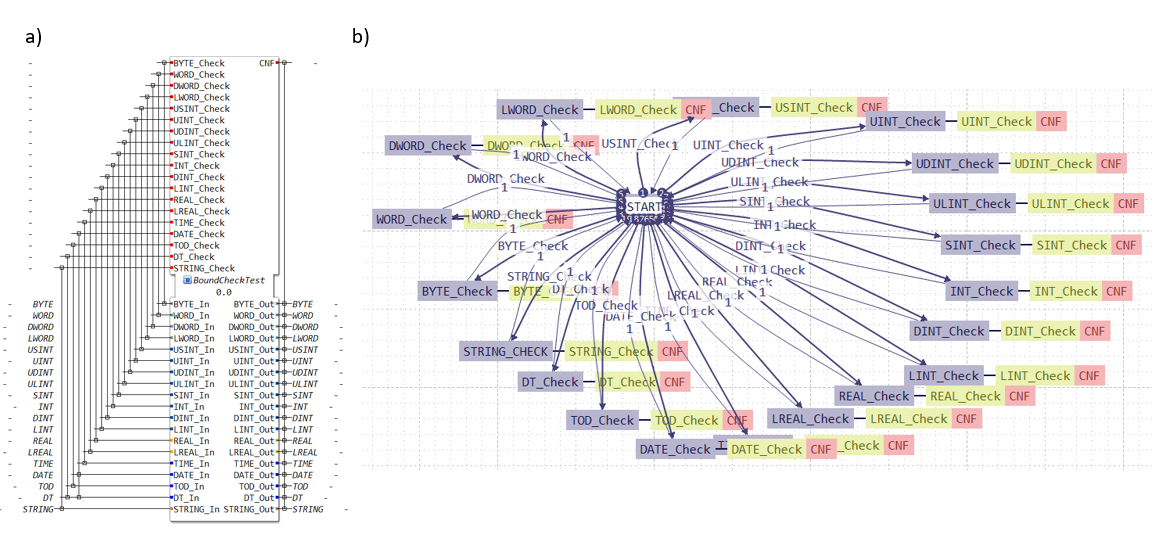
\includegraphics[width=1\textwidth]{Figures/BCT4Diac.PNG}
	\caption{BoundCheckTest FB a) Interface b) ECC}
	\label{fig:BCT4Diac}
\end{figure*}


BoundCheckTest FB \ref{fig:BCT4Diac} is a test function block that tests the boundary support for each data type such as BYTE, WORD, DWORD, LWORD, USINT, UINT, UDINT, ULINT, SINT, INT, DINT, LINT, LREAL, TIME, DATE, TOD, STRING. This function block can be used to check if the system under test can handle the maximum and minimum values of the specified data types correctly.

To test the BoundCheckTest function block, input data needs to be added with necessary values and then the bound check event for the specified data type should be triggered. The output values of the event should be the input value plus one. For example, if the input value is In1, the output value should be Out1 = In1 + 1. This will also trigger the CNF event, indicating that the test has been completed successfully.

The purpose of the BoundCheckTest is to ensure that the system under test can handle the maximum and minimum values of the specified data types without any errors or unexpected behavior. This is important because it ensures the reliability and robustness of the system, especially in situations where the system is required to handle extreme values.


\begin{figure}[!b]
    \centering
    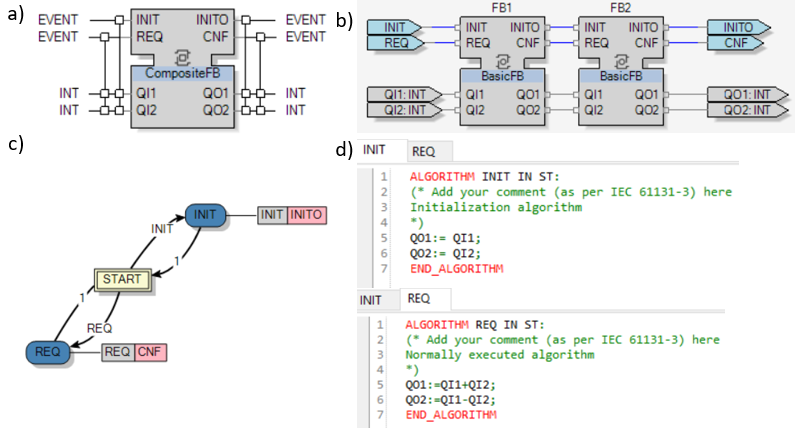
\includegraphics[width=\columnwidth]{Figures/CFBTest.PNG}
    \caption{a) Composite Function Block a) FB interface b) Basic FB connection Diagram c) ECC d) INIT Algorithm and REQ Algorithm.} 
    \label{fig:CFBTest}
\end{figure}

\begin{figure}[!b]
    \centering
    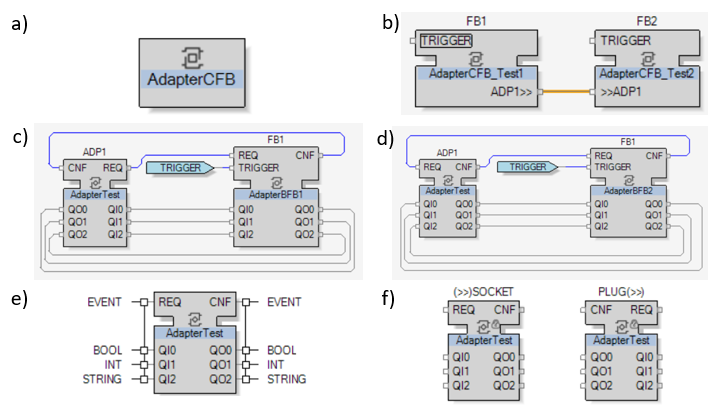
\includegraphics[width=\columnwidth]{Figures/AdapterCFB.PNG}
    \caption{ shows the Function Block Interface of a) Adapter CFB b) AdapterCFB consists of two sub-CFBs i.e. AdapterCFB\_Test1 and AdapterCFB\_Test2 c) AdapterCFB\_Test1 consists of AdapterTest FB and an AdapterBF1 (basic FB) d)  AdapterCFB\_Test2 consists of AdapterTest FB and an AdapterBF1 (basic FB), e \& f) Represents the  AdapterTest FB  and its SOCKET and PLUG } 
    \label{fig:AdapterCFB}
\end{figure}

\subsection{StanadardFunctionTest FB}

The StandardFunctionTest FB is designed to evaluate the support of IEC 61499 standard functions and their corresponding association with input values. This FB is capable of testing over 75 standard functions by providing specific events for testing each function, which trigger the corresponding testing algorithm for that particular function.

To test the StandardFunctionTest function block, suitable input values are added to the input data, and the function event is triggered. The output values should contain the result of the corresponding function, which is then verified by the CNF event.

For instance, if In1 is the input value, the output value Out1 should be equal to the result of the function evaluated using In1. Therefore, the CNF event confirms that the expected output value is produced. Let's consider the following example to test the MUX function feature,


To test the Multiplexer (MUX) function, the MUX\_Func event should be triggered, and the corresponding algorithm will execute.

\begin{lstlisting} 
ALGORITHM MUX_Func IN ST:
(* Add your comment (as per IEC 61131-3) here
*)
MUX_Out:=MUX(int1,time1,time2,time3);
END_ALGORITHM
\end{lstlisting}




The MUX function is used to select one of several input signals based on an index value. The input signals can be of different types, such as time, integers, etc. The MUX function returns the selected input signal based on the index value. The MUX function can be tested by triggering the MUX\_Func event and verifying that the output value matches the expected output value.

If we provide input values int1=2, time1=TIME\#1m30s, time2=T\#15s, and time3=T\#2m30s, then the expected output is MUX\_Out:=MUX(int1,time1,time2,time3) = 2m30s.


\subsection{CompositeBlockTest}

The CompositeBlock FB \ref{fig:CFBTest} is used to test the functionality of composite function block support. The block has two events, INIT and REQ, which can be triggered in manual testing mode or by adding integer values to the input data and triggering the REQ event.

When the INIT event is triggered, the output values should be the same as the input values, and the INITO event is fired. On the other hand, when the REQ event is triggered, the output should be calculated as QO1 = QI1 + QI2 and QO2 = QI1 - QI2. After the calculation is complete, the CNF event is fired.

In summary, the CompositeBlock function block tests the functionality of composite function blocks by calculating the output values based on the input values and triggering the CNF event when the calculation is complete.

\subsection{AdapterTest CFB}


AdapterCFB \ref{fig:AdapterCFB} is a function block that tests the functionality of adapter support. The AdapterCFB is composed of two basic function blocks, AdapterBFB1 and AdapterBFB2. AdapterBFB1 has three output parameters, QO0, QO1, and QO2, which are initialized to FALSE, 1, and "AdapterBFB1", respectively. AdapterBFB2 also has three output parameters, QO0, QO1, and QO2, which are initialized to TRUE, 2, and "AdapterBFB2", respectively.

The input values from AdapterBFB1 are transferred to AdapterBFB2 and vice versa. This is made possible through the use of an adapter, which connects the two function blocks. When the AdapterCFB is triggered, the input values are set by the tester, and the output values are calculated by the adapter based on the input values.

In other words, AdapterCFB provides a way to connect two function blocks that have different inputs and outputs by mapping the inputs and outputs of one block to the inputs and outputs of the other block, using an adapter.

\section{Xml-import/export compatibility test
between 4DIAC  V2.0.1 and EAE 
V21.2}

As a part of the 1-Swarm project, a hackathon was conducted to analyze the compatibility of IEC 61499 between 4DIAC and Schinder Electric EcoStruxure (EAE). The objectives of the hackathon were to identify portability issues between 4DIAC and EAE-IDE, as well as between Forte and EcoRT-runtime, create a roadmap for addressing the identified issues, and discuss potential solutions for creating a single portable test application that can automatically test new versions of IDE and runtime and certify some key attributes. Some of the issues identified during the hackathon are given below: 

\begin{enumerate}

\item Issue: The EAE import dialog does not allow for the selection of a $<BitStringDataType.Basic.ZIP>$ named file with a subdirectory IEC61499 and a metafile named $<BitStringDataType.Basic.export>$. EAE requires a specific extended import format which is not described in the IEC61499 standard.

Recommendation: Develop a company conformance profile or allow for the import of pure .fbt files to address the issue.

\item  Issue: After importing a 4diac .xml file in the 4DIAC .BASIC.ZIP format, the algorithms are not imported. EAE does not accept the CDATA format for the textual contents of algorithms.

Recommendation: Modify EAE to accept CDATA format as it offers user format overall lines, instead of compressing the algorithm in one .xml line.

\item Issue: The compiler/parser does not generate an error when a function with two parameters is called with only one argument.

Recommendation: Modify the compiler/parser to generate an error when an argument is missing.


\item Issue: EAE does not support data types CHAR, WCHAR, and WSTRING. Only the STRING data type is supported.

Recommendation: Modify EAE to support character string literals that directly represent a character or character string value of data type CHAR, WCHAR, STRING, or WSTRING as documented in the IEC61131-3 standard.
\end{enumerate}

An automated testing approach for assessing the compatibility of software tools and runtime platforms with the IEC 61499 standard could be a promising direction for future research and development. This approach could leverage service sequence testing as an additional testing methodology to ensure comprehensive compliance with the IEC 61499 specification across all integrated development environments (IDEs) and runtime environments. 

\section*{Acknowledgment}
This work was sponsored, in part, by the H2020 project 1-SWARM co-funded by the European Commission (grant agreement: 871743). Thank you Artur Fritz and Alois Zoitl for their valuable contributions and participation in the hackathon for the development of the IEC 61499 portability test suite.

\bibliographystyle{IEEEtran}
\bibliography{conference.bib}


\end{document}
